\documentclass{article}
\usepackage{tikz}
\usepackage{pgf-umlcd}
\begin{document}
\section*{Clase Address Translation Architecture}
\begin{center}
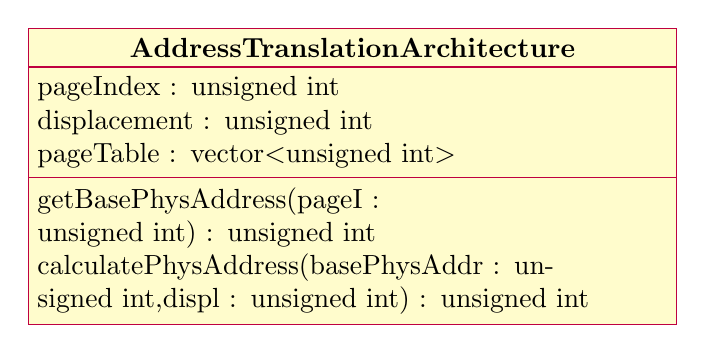
\begin{tikzpicture}
  \begin{class}[text width=8cm]{AddressTranslationArchitecture}{0,0}
    %\attribute{N : unsigned int}
    \attribute{pageIndex : unsigned int}
    \attribute{displacement : unsigned int}
    \attribute{pageTable : vector$<$unsigned int$>$}    
    \operation{getBasePhysAddress(pageI : unsigned int) : unsigned int}
    \operation{calculatePhysAddress(basePhysAddr : unsigned int,displ : unsigned int) : unsigned int}
    % virtual operations
    %\operation[0]{name(parameters list) : type of value returned}
    %\operation[0]{calcularArea() : void}
  \end{class}
\end{tikzpicture}
\end{center}
\begin{verbatim}
/**AddressTranslationArchitecture.h*/
#ifndef ATA_H
#define ATA_H
struct AddressTranslationArchitecture{
  unsigned int pageIndex;
  unsigned int displacement;
  vector<unsigned int> pageTable;
  
  unsigned int getBasePhysAddress(unsigned int pageI);
  unsigned int calculatePhysAddress(
               unsigned int basePhysAddr,
               unsigned int displ);
};/*end struct AddressTranslationArquitecture*/
#endif /*ATA_H*/

/**AddressTranslationArchitecture.cpp*/
#include <AddressTranslationArchitecture.h>

unsigned int AddressTranslationArchitecture::calculatePhysAddress(
             unsigned int basePhysAddr,unsigned int displ){
  return (basePhysAddr+displ);                                  
}

unsigned int AddressTranslationArchitecture::getBasePhysAddress(
             unsigned int pageI){
  return pageTable[pageI];
}
\end{verbatim}
\end{document}